
\chapter{Equivalent Circuits}

In this lab, you will explore Thevenin equivalent circuits. You will
also solder two resistor circuits to explore the $\Delta$-$Y$
transformation for three terminal networks. For this lab, both logbook
and Jupyter Notebook entries are required. You can find the resistors
inside storage cabinet at the table to your left and cables hanging at
the wall to your left. Please return them at the end of the lab.

\section{Calculations}

\noindent
During lecture we determined an equation for the Thevenin
equivalent voltage $V_{\rm th}$ and resistance $R_{\rm th}$ from the
values $V_1, V_2, R_1, R_2, R_3$ for the circuit shown in
Fig.~\ref{fig:thevenin}.
%Hint: Use the superposition principle. Find the equivalent resistance
%by setting the voltage $V_1$ and $V_2$ to zero, i.e. shorting them in
%the circuit.  Then calculate two contributions to the Thevenin
%voltage, one with $V_1$ set to zero and one with $V_2$ set to zero.
%The actual Thevenin voltage is the sum of these two contributions.
%Play close attention to the polarity of $V_2$ as drawn, i.e. that a
%positive value of $V_2$ tends to make the voltage $V_{\rm a b}$
%negative.

\begin{measurement} 
Repeat this calculation in terms of $V_1, V_2, R_1, R_2, R_3$ in your
logbook together with the sketch of the circuit.
\end{measurement}

\begin{figure}[htbp]
\begin{center}
\begin{tabular}{c@{\hskip 2cm}c}
\begin{circuitikz}[line width=1pt]
\draw (0,0) to[voltage source,bipoles/length=1.5cm,l=$V_1$,invert] ++(0,2.0)
coordinate(X) to[R,l=$R_3$,-*] ++(2.0,0); \draw (X) to[R,l=$R_1$]
++(0,2.0) to[short,-*] ++ (2.0,0) coordinate(X) to[short,-o] ++
(1.0,0) node[right]{B}; \draw (X) to[voltage
  source,bipoles/length=1.5cm, l=$V_2$,invert] ++(0,-2.0) to[R,l=$R_2$]
++(0,-2.0) coordinate(X) to[short,*-o] ++ (1.0,0) node[right]{A};
\draw(X) to[short] ++(-2.0,0);
\end{circuitikz} &
\begin{circuitikz}[line width=1pt]
\draw (0,0) coordinate(X) to[voltage source,bipoles/length=1.5cm,l=$V_{\rm th}$,invert] ++(0,2.0) to[R,l=$R_{\rm th}$,-*] ++(0,2.0)
to[short,-o] ++ (3.0,0) node[right]{B};
\draw(X) to[short,-o] ++ (3.0,0) node[right]{A};
\end{circuitikz} \\
(a) & (b) \\
\end{tabular}
\caption{The circuit (a) you will be building in lab and it's (b) Thevenin Equilvalent.}
\label{fig:thevenin}
\end{center}
\end{figure}

\section{Thevenin Equivalent Circuit}

Build the circuit (on a breadboard) in Fig.~\ref{fig:thevenin} using $R_1 = 3.3~\rm
k\Omega$, $R_2 = 3.9~\rm k\Omega$, and $R_3 = 4.7~\rm k\Omega$.
Supply $V_1 = 10~\rm V$ and $V_2 = 5~\rm V$ using your two channel
bench-top power supply.  In the diagram, the supplies are not
referenced to ground or each other, so make certain that your supply
is set to provide independent outputs and do not add any jumpers to
ground.  Take careful note of the polarity of the supplies, so
e.g. the negative (black) output of $V_1$ is connected to point (A)
whereas the negative (black) output of $V_2$ is connected to point
(B).Use your Triplett 9007 as a voltmeter and the Mastech MS8624 as a
current meter.   

\begin{measurement} 
Compute $V_{\rm th}$, $R_{\rm th}$, and the short-circuit current
$I_{\rm sc}$ for the particular values of $R_1$,$R_2$,$R_3$,$V_1$, and
$V_2$ you will be using in the lab. Record these values in your logbook.  
\end{measurement}

\begin{measurement} 
First measure the open circuit voltage $V_{\rm ab}$.  Next short the
points (a) and (b) through your current meter. Record these values in
your logbook.  These values should closely match the Thevenin voltage
and short-circuit current which you have already calculated.  If not,
you should check your work and find the discrepancy before
proceeding. Record your comments in the logbook.
\end{measurement}

\begin{measurement}  
Next you will measure the voltage across and current through a load
resistor connected between the terminals at (A) and (B) to
experimentally determine the IV curve for your circuit.  Recall from
the previous lab that you measure the current by connecting your meter
in series and the voltage by connecting your meter in parallel.  As
before, use your Triplett 9007 as a voltmeter and the Mastech MS8624
as a current meter. Make simultaneous current and voltage measurements
for three different values of the load resistance $R = 470~{\rm
  \Omega}, 1.2~\rm k\Omega, 4.7~\rm k\Omega.$ Record these values in
your logbook.
\end{measurement}

\section{Analysis}

\begin{plot}
To present your analysis you should produce a plot similar to that of
Fig.~\ref{fig:egthev}.  Your plot should show the Thevenin equivalent
source IV curve for the circuit you built in lab.  You should also
draw theoretical load IV curves for the three resistor values you used
to make current and voltage.  Finally, you should include data points
for the five current and voltage measurements which you have made.
\end{plot}

\begin{figure}[htbp]
\begin{center}
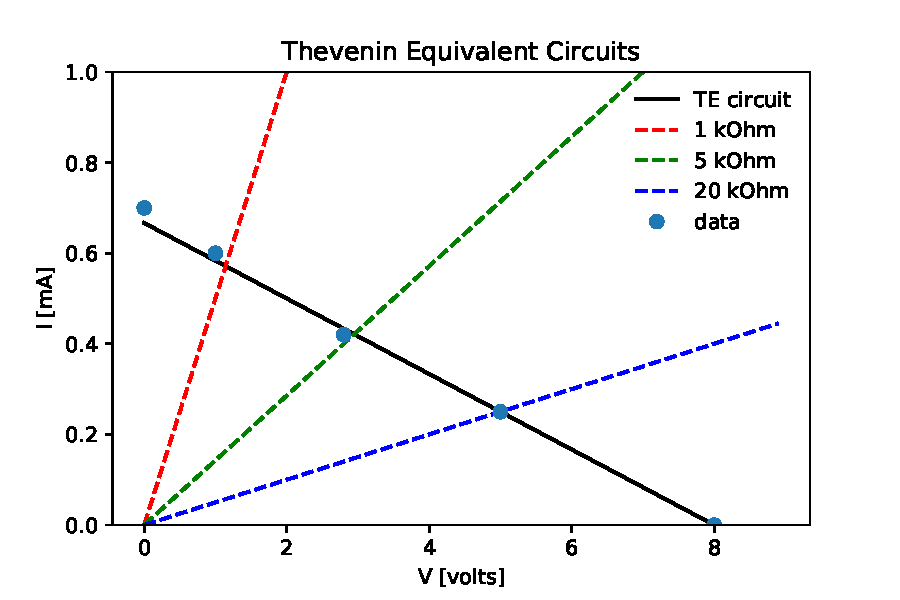
\includegraphics[width=0.75\textwidth]{figs/labs/thevenin/final.pdf} 
\caption{Example of IV curves for Thevenin equivalent source circuit with various load resistors. }
\label{fig:egthev}
\end{center}
\end{figure}

\section{Impact of the Multimeter on the Measured Circuit}

A perfect DMM would not affect the circuit you are measuring at all,
but this is not the case in practice. An ideal voltmeter has infinite
resistance so that it draws zero current when measuring voltage across
two points. An ideal ammeter has zero resistance so that there is no
voltage change as the current passes through it.  Your DMM has a small
non-zero resistance when used as an ammeter, and a large resistance
when used as a voltmeter.

\begin{measurement} 
Build the voltage divider of Fig.~\ref{fig:dividers}a but with
$V_1=10~\rm{V}$ and $R_1 = R_2 = 10~\rm{M\Omega}$. Record the voltage
across one of the resistors. Compare the value your measure with what
you predict for a perfect DMM. Sketch the circuit with a realistic DMM
and calculate the resistance of your DMM when used as a voltmeter.
\end{measurement}

\noindent
This is a \textbf{sign-off point} for this lab. 

\section{$\Delta-Y$ Transformation}

Not everyone will complete this portion of the lab.  Do your best to
finish as much as you can.

\begin{figure}[htbp]
\begin{center}
\begin{tabular}{c@{\hskip 2cm}c}
\begin{circuitikz}[line width=1pt]
\draw (0,0) coordinate(A);
\draw (A) to[R,l_=$R_A$,*-*] ++(0,2.0) node[above]{A};
\draw (A) to[R,*-*] ++(-1.73,-1) node[left]{B};
\draw (A) to[R,*-*] ++(1.73,-1) node[right]{C};
\draw (-0.5,0) node[left]{$R_B$};
\draw (1.25,0) node[left]{$R_C$};

\end{circuitikz} &
\begin{circuitikz}[line width=1pt]
\draw (0,2) to [R] (1.73,-1) node[right]{C} to [R,*-,l_=$R_{BC}$] (-1.73,-1) node[left]{B} to [R,*-*] (0,2) node[above]{A};
\draw (-0.75,1) node[left]{$R_{AB}$};
\draw (0.8,1) node[right]{$R_{AC}$};
\end{circuitikz} \\
(a) & (b) \\
\end{tabular}
\caption{Equivalent three-node circuits.}
\label{fig:deltay}
\end{center}
\end{figure}

Consider the two different networks shown in Fig.~\ref{fig:deltay}.
If there are no external connections to the central node in the
left-hand circuit, the two networks are equivalent if:
\begin{displaymath}
R_{A} = \frac{R_{AC} R_{AB}}{R_{AB} + R_{AC} + R_{BC}}
\end{displaymath}
as well as two similar equations for $R_{B}$ and $R_{C}$.  Going in the other direction we have:
\begin{displaymath}
R_{AB} = \frac{R_{A}R_{B} + R_{A}R_{C} + R_{B}R_{C}}{R_{C}}.
\end{displaymath}
These transformations are more general than the series and parallel
laws, which you can derive by considering the case that $R_{BC}=0$ for
parallel resistors, and $R_{C} \to \infty$ for series resistors.  They
allow one to simplify more complicated networks for which the series and
parallel equivalence relations are insufficient.

In the special case that $R_{A} = R_{B} = R_{C} = R$ it follows that 
\begin{displaymath}
R_{AB} = R_{AC} = R_{BC} = 3 R.
\end{displaymath}

Use your soldering iron to construct the left-hand network using
$R_{A} = R_{B} = R_{C} = 1~\rm k\Omega$.  Then construct the
equivalent right-hand network using $R_{AB} = R_{AC} = R_{BC} =
3.0~\rm k\Omega$.  If $3~\rm k\Omega$ resistors are not available, you
can construct one by using a $33~\rm k\Omega$ in parallel with a
$3.3~\rm k\Omega$ resistor.

Make sure the soldering iron is on, and the sponge is moist.  There is
one soldering iron per two workstation. Find the squeeze bottle around
the lab. The clamps (possibly various styles) are on the shelves to
your left. Twist the leads of the resistor together to make initial
connections, then hold the arrangement securely in the clamp.  Wipe
the tip of the hot iron on the sponge to clean it, then apply a small
amount of solder to the tip by touching the hot iron to the solder
wire.

Heat the connection by holding the soldering iron against it, then
bring the solder wire in contact with the heated connection (not the
soldering iron) You want the iron to heat the connection, and then the
connection to melt and draw in the solder.  The little bit of solder
on the tip is only there to ensure good thermal conduct between the
tip and the connection: don't ``paint'' the solder onto the
connection.

\begin{measurement} 
Check the resistance between pairs of terminals on your creations, and
compare with your expectation. Record those values in your logbook. You can bring your creations home if
you like or bring them to the front desk. 
\end{measurement}

This is an additional \textbf{sign-off point} for this lab. 

\noindent
Please return all the components you took and cables to their place. Leave you workstation clean. 

